\section{Data Exploration\label{sec:dataexploration}}

Upon exploring the data three main characteristics appeared. Below we explore each a bit more. 

\mysubsection{Review Distribution}
The data set consists of 50.000 reviews and their corresponding review rating (1-4 for negative, 7-10 for positive). 
In Figure~\ref{fig:data-dist} the split for both the training and test set can be found.
It can be noted that the distributions are about the same, meaning the data set does not have an inherent bias towards positive or negative reviews.
Another interesting fact is that both review of score 1 and 10 are highly represented in the data set in comparison to the other review scores.

\begin{figure}[ht!]
    \centering
  \subfloat[Test Review Distribution\label{fig:test-dist}]{%
       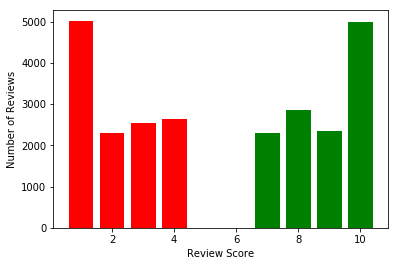
\includegraphics[width=0.5\linewidth]{figures/data-visualization/test_review_dist.png}}
    \hfill
  \subfloat[Train Review Distribution\label{fig:train-dist}]{%
        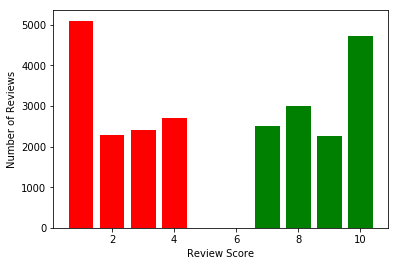
\includegraphics[width=0.5\linewidth]{figures/data-visualization/train_review_dist.png}}
  \caption{Test \ref{fig:test-dist} and train \ref{fig:train-dist} review frequency distribution.}
  \label{fig:data-dist} 
\end{figure}

\mysubsection{Binary Classification}
Even though the data has multiple bins, we will in the end classify the data in two bins: (1) positive or (2) negative. Binary classification has an impact on which classifiers are used, and the parameters that are chosen. 

The 2-dimensional representation of the training and testing datasets, using Latent Semantic Analysis (LSA), is shown in Figure~\ref{fig:data-2d-vis}. We reduced the dimensions by first fitting LSA onto the training data. After that we transformed both data sets. What we can see is that for the training data, see Figure~\ref{fig:train-2d-lsa}, that the data becomes almost separable with a few errors. However, for the test data, see Figure~\ref{fig:test-2d-lsa}, this is clearly not the case. Both classes are randomly distributed among each other, making classifying very difficult. We can conclude that the data is not linearly separable.

\begin{figure}[ht!]
    \centering
  \subfloat[Train data set using SVD\label{fig:train-2d-svd}]{%
       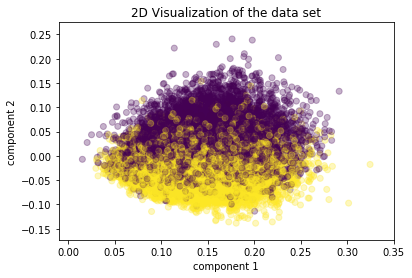
\includegraphics[width=0.5\linewidth]{figures/data-visualization/2d-data-visualization-train-svd.png}}
    \hfill
  \subfloat[Test data set using SVD\label{fig:test-2d-svd}]{%
        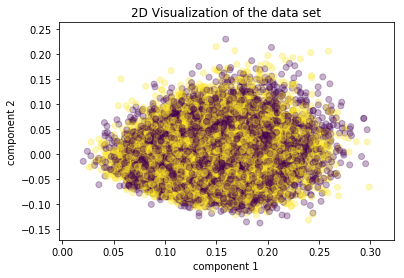
\includegraphics[width=0.5\linewidth]{figures/data-visualization/2d-data-visualization-test-svd.png}}
        
    \subfloat[Train data set using LSA\label{fig:train-2d-lsa}]{%
        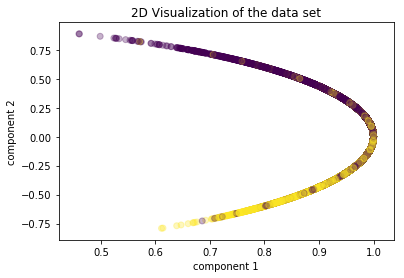
\includegraphics[width=0.5\linewidth]{figures/data-visualization/2d-data-visualization-train-lsa.png}}
    \hfill
    \subfloat[Test data set using LSA\label{fig:test-2d-lsa}]{%
        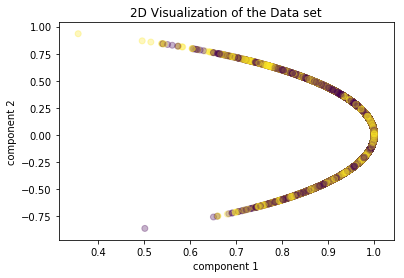
\includegraphics[width=0.5\linewidth]{figures/data-visualization/2d-data-visualization-test-lsa.png}}
  \caption{2D visualization of the data using dimensionality reduction (LSA)}
  \label{fig:data-2d-vis} 
\end{figure}

\mysubsection{Word Clouds}
When looking at the reviews and analyze the positive and negative reviews separately, we can see that the distribution of words differ, but many appear in both data sets, see Figure~\ref{fig:wordclouds}.
This can be an indication that just using the term-frequency may not be the best feature out there.
Solely, based on the word clouds it is tough to distinguish which cloud describes the positive or negative reviews.

Moreover the size of the reviews varied as well. Maximum amount of reviews ranged between 200-300 words. This was essential to find as we persist word vectors and different inputs in the neural networks. We padded the reviews accordingly.

\begin{figure*}[ht!]
    \centering
  \subfloat[Negative word cloud\label{fig:neg-wordcloud}]{%
       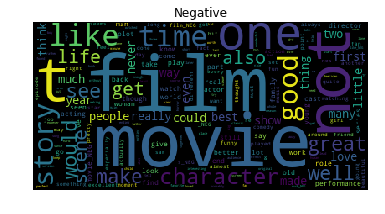
\includegraphics[width=0.5\linewidth]{figures/data-visualization/negative_wordcloud.png}}
    \hfill
  \subfloat[Positive word cloud\label{fig:pos-wordcloud}]{%
        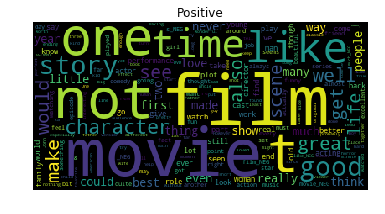
\includegraphics[width=0.5\linewidth]{figures/data-visualization/positive_wordcloud.png}}
  \caption{Word clouds for the both negative \ref{fig:neg-wordcloud} and positive \ref{fig:pos-wordcloud} reviews.}
  \label{fig:wordclouds} 
\end{figure*}